\documentclass{article}
\usepackage{fancyhdr}
\usepackage{amsmath,amssymb}
\usepackage{geometry}
\usepackage{datetime}
\usepackage{enumerate}
\usepackage{graphicx}

%Insert page formatting here
\hoffset = -.5in
\voffset = -0.375in
\textwidth = 7in
\textheight = 8in
\headheight = 24pt

\pagestyle{fancy}

\rhead{Peter Olson\\Student ID: $441666$}
\lhead{Math 3200\\Homework 10}
\chead{\today}
\cfoot{}

%\addtolength{\headwidth}{\marginparsep}
%\addtolength{\headwidth}{\marginparwidth}

%\renewcommand{\labelitemi}{$\diamond$}
\renewcommand{\implies}{\rightarrow}
\newcommand{\widespace}{\qquad \qquad \;}
\newcommand{\tret}{\\ \hline}
\newcommand{\fh}{\tfrac{1}{2}}
\newcommand{\deriv}[2]{\frac{d #1}{d #2}}
\newcommand{\pderiv}[2]{\frac{\delta #1}{\delta #2}}
\newcommand{\vr}{\vec{r}}
\newcommand{\at}{\text{ at }}
\newcommand{\var}{\text{Var}}
\newcommand{\cov}{\text{Cov}}

\begin{document}

\section*{Exercise 10.22}

\begin{enumerate}[\quad(a)]
	\item Make four plots and comment on their linearity.
	\begin{center}
		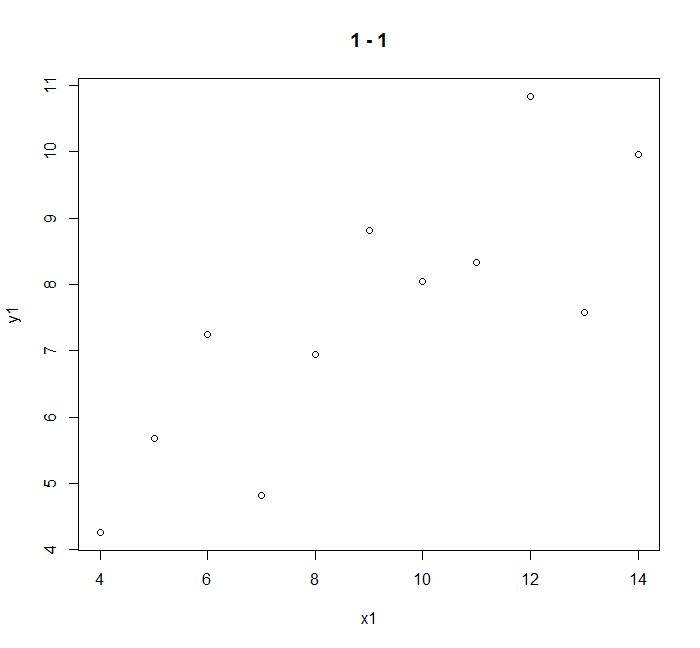
\includegraphics[width=3in]{Q61.png}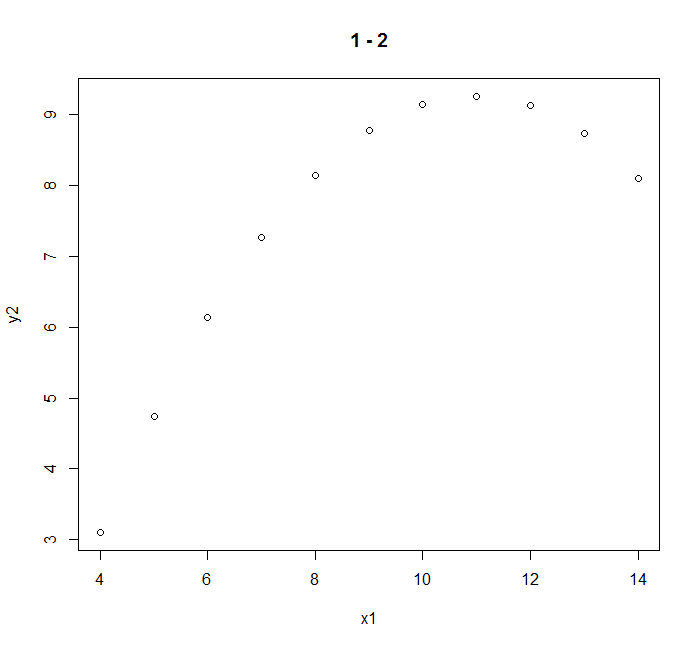
\includegraphics[width=3in]{Q62.png}
		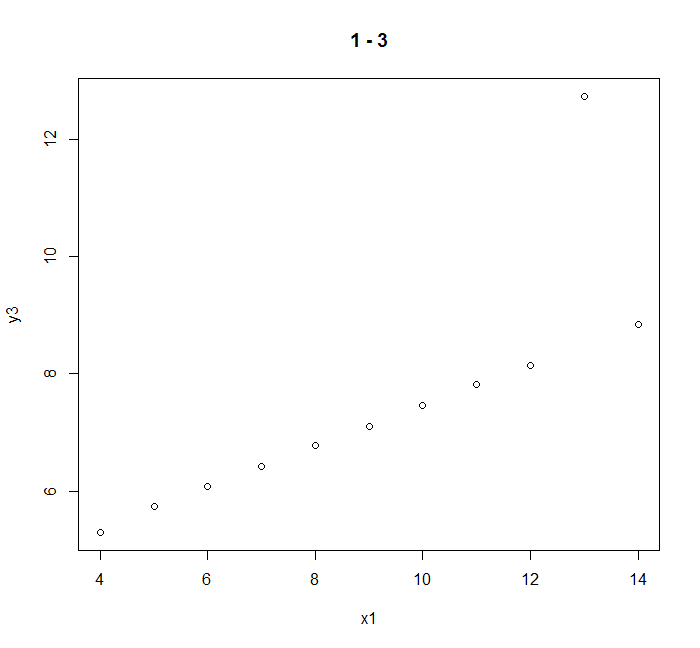
\includegraphics[width=3in]{Q63.png}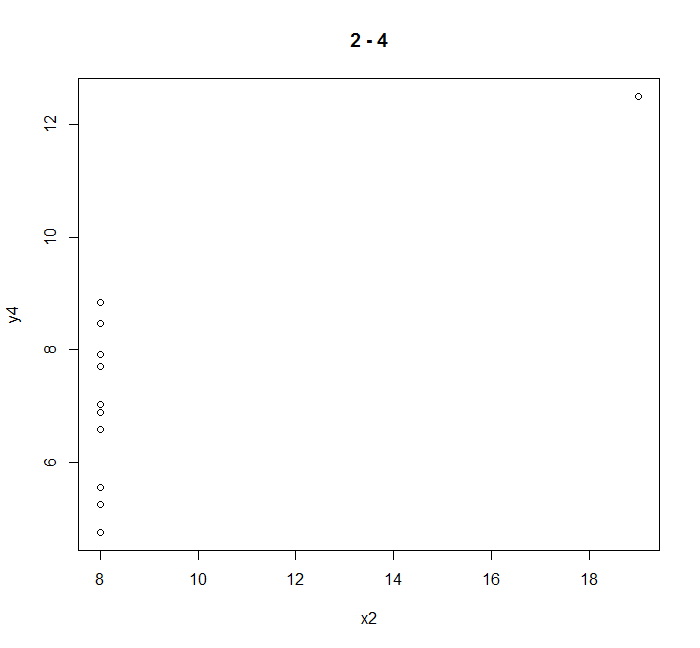
\includegraphics[width=3in]{Q64.png}
	\end{center}
	1 - 1 appears to be a mostly random data set. 1 - 2 appears parabolic, which isn't even close to linear.
	1 - 3 appears almost perfectly linear, save for a single outlier. 2 - 4 looks almost vertical, which suggest a very strange relationship, with one far outlier.

	\newpage
	\item Fit LS straight lines to the four plots and compute the usual statistics that accompany the LS fits. Note that the numerical results are identical.
	\begin{center}
		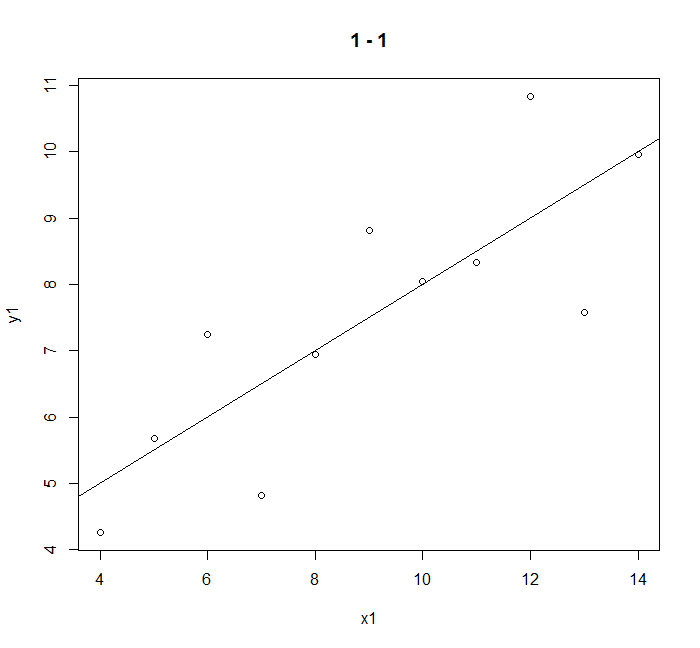
\includegraphics[width=3in]{Q65.png}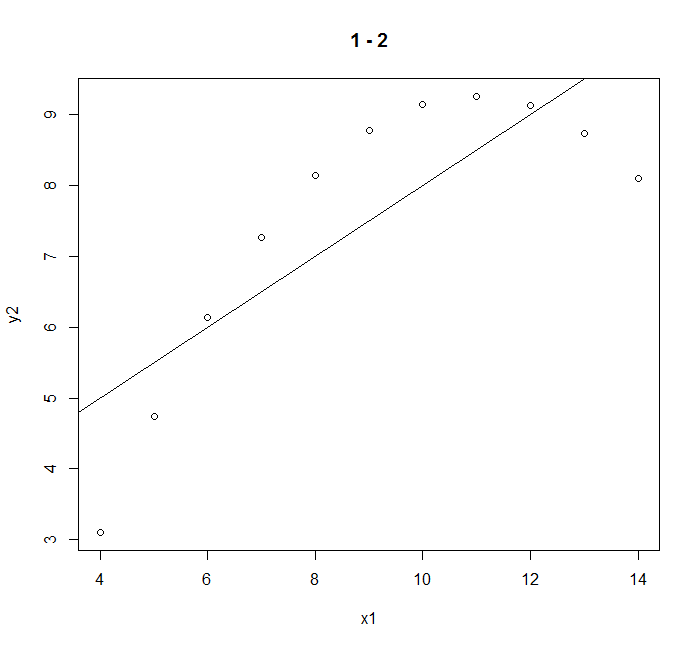
\includegraphics[width=3in]{Q66.png}
		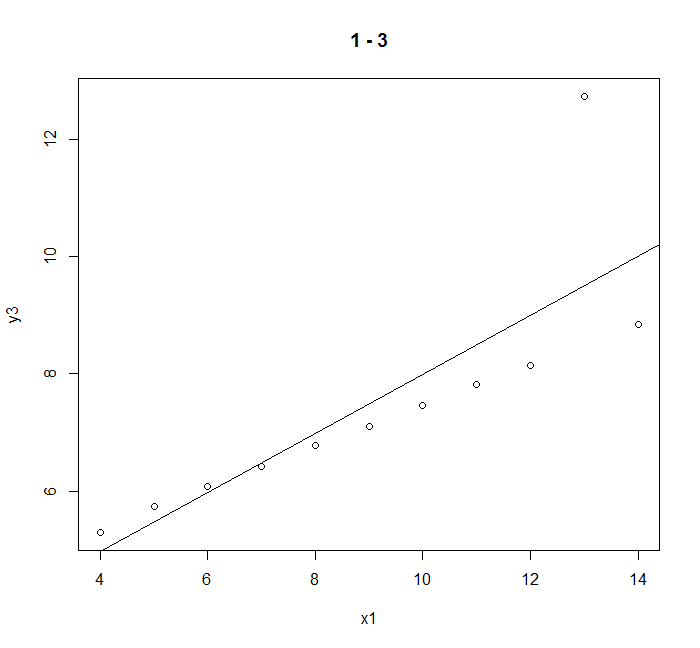
\includegraphics[width=3in]{Q67.png}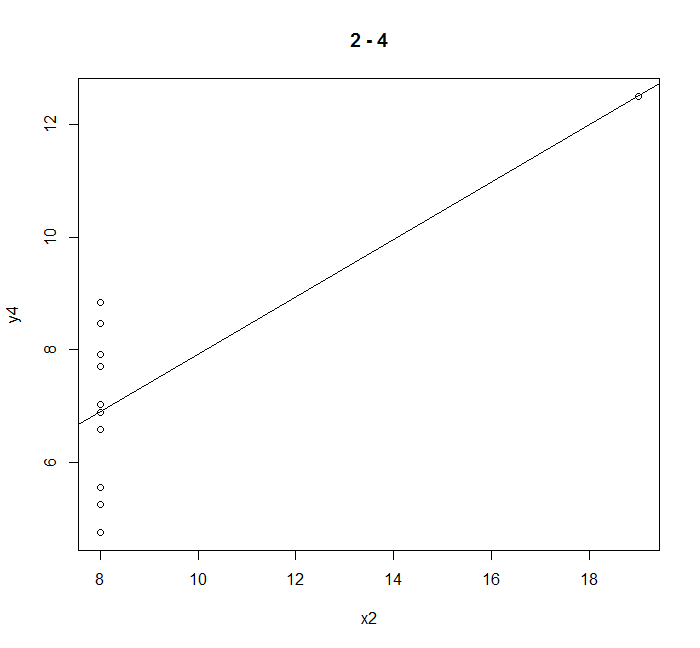
\includegraphics[width=3in]{Q68.png}
	\end{center}

	While it is true that they have very similar fits, the F-statistics are very different for the fits.

	\item The reason they're they same is because each of the sets contiains outliers placed in just the right place so that, when they're summarized by a LS fit, they wind up giving the same fit. This is because any fit is an extrapolation on the data, and the actual nature of the dataset is being approximated. Therefore, one would very much benefit from plotting a dataset first, before running fits on it.

	\item This shows that these test statistics ($r^2$ and $t$) are just, again, approximations of the linear fit, and not necessarily as descriptive as one might hope they are for the absolute last word on a particular dataset's linearity.
\end{enumerate}

\section*{R Code}
\begin{verbatim}
# set up data
x1 <- c(
  10, 8, 13, 9,
  11, 14, 6, 4,
  12, 7, 5
)
y1 <- c(
  8.04, 6.95, 7.58, 8.81,
  8.33, 9.96, 7.24, 4.26,
  10.84, 4.82, 5.68
)
y2 <- c(
  9.14, 8.14, 8.74, 8.77,
  9.26, 8.10, 6.13, 3.10,
  9.13, 7.26, 4.74
)
y3 <- c(
  7.46, 6.77, 12.74, 7.11,
  7.81, 8.84, 6.08, 5.29,
  8.15, 6.42, 5.73
)
x2 <- c(
  8, 8, 8, 8,
  8, 8, 8, 19,
  8, 8, 8
)
y4 <- c(
  6.58, 4.76, 7.71, 8.84,
  8.47, 7.04, 5.25, 12.50,
  5.56, 7.91, 6.89
)

# a
plot(x1,y1, main = " 1 - 1 ")
plot(x1,y2, main = " 1 - 2 ")
plot(x1,y3, main = " 1 - 3 ")
plot(x2,y4, main = " 2 - 4 ")

# b
fit1 = lm(y1~x1)
fit2 = lm(y2~x1)
fit3 = lm(y3~x1)
fit4 = lm(y4~x2)

plot(x1,y1, main = " 1 - 1 ")
abline(fit1)
plot(x1,y2, main = " 1 - 2 ")
abline(fit2)
plot(x1,y3, main = " 1 - 3 ")
abline(fit3)
plot(x2,y4, main = " 2 - 4 ")
abline(fit4)

# print r^2
sqrt(sum(resid(fit1)^2) / (length(x1) - 2))
sqrt(sum(resid(fit2)^2) / (length(x1) - 2))
sqrt(sum(resid(fit3)^2) / (length(x1) - 2))
sqrt(sum(resid(fit4)^2) / (length(x1) - 2))

# print summaries

summary(fit1)[['coefficients']]
summary(fit2)[['coefficients']]
summary(fit3)[['coefficients']]
summary(fit4)[['coefficients']]

summary(fit1)[['fstatistic']]
summary(fit2)[['fstatistic']]
summary(fit3)[['fstatistic']]
summary(fit4)[['fstatistic']]
\end{verbatim}

\section*{R Output}
\begin{verbatim}
> # print r^2
> sqrt(sum(resid(fit1)^2) / (length(x1) - 2))
[1] 1.236603

> sqrt(sum(resid(fit2)^2) / (length(x1) - 2))
[1] 1.237214

> sqrt(sum(resid(fit3)^2) / (length(x1) - 2))
[1] 1.233121

> sqrt(sum(resid(fit4)^2) / (length(x1) - 2))
[1] 1.379392

> # print summaries
> summary(fit1)[['coefficients']]
             Estimate Std. Error  t value    Pr(>|t|)
(Intercept) 3.0000909  1.1247468 2.667348 0.025734051
x1          0.5000909  0.1179055 4.241455 0.002169629

> summary(fit2)[['coefficients']]
            Estimate Std. Error  t value    Pr(>|t|)
(Intercept) 3.000909  1.1253024 2.666758 0.025758941
x1          0.500000  0.1179637 4.238590 0.002178816

> summary(fit3)[['coefficients']]
             Estimate Std. Error  t value    Pr(>|t|)
(Intercept) 2.9524545  1.1215793 2.632408 0.027250845
x1          0.5042727  0.1175735 4.289001 0.002023035

> summary(fit4)[['coefficients']]
            Estimate Std. Error  t value    Pr(>|t|)
(Intercept)    2.829  1.2546192 2.254867 0.050599229
x2             0.509  0.1315198 3.870139 0.003787965

> summary(fit1)[['fstatistic']]
   value    numdf    dendf 
17.98994  1.00000  9.00000 

> summary(fit2)[['fstatistic']]
   value    numdf    dendf 
17.96565  1.00000  9.00000 

> summary(fit3)[['fstatistic']]
   value    numdf    dendf 
18.39553  1.00000  9.00000 

> summary(fit4)[['fstatistic']]
   value    numdf    dendf 
14.97798  1.00000  9.00000 
	\end{verbatim}

\end{document}